%%% use twocolumn and 10pt options with the asme2ej format
\documentclass[twocolumn,10pt]{asme2ej}
\usepackage{amssymb}
\usepackage{amsmath}
\usepackage{epsfig} %% for loading postscript figures
\usepackage{graphicx}
\usepackage{algorithm}
\usepackage{algorithmicx, float}
\usepackage{algpseudocode}

\title{De-Mystifying Reduced-Order St. Venant-Kirchhoff Deformable Models}

\author{Gillian P. Reyes
}

\begin{document}

\maketitle

% %%%%%%%%%%%%%%%%%%%%%%%%%%%%%%%%%%%%%%%%%%%%%%%%%%%%%%%%%%%%%%%%%%%%%%
\begin{abstract}
{\it The goal of this paper is to document each step taken in recreating
the results of Real-Time Subspace Integration for St. Venant-Kirchhoff Deformable Models \cite{barbic}, so that
others may use this as a guide to replicate this work.
}
\end{abstract}

% %%%%%%%%%%%%%%%%%%%%%%%%%%%%%%%%%%%%%%%%%%%%%%%%%%%%%%%%%%%%%%%%%%%%%%
\section{Introduction}

The goal of this paper is to document each step taken in recreating Barbič and James's research from their 2005
paper \cite{barbic}. In this research, they utilize past work on real-time deformable objects and model reduction in solid mechanics to speed up computations and allow for large deformations. Finite Element Method is used to discretize partial differential equations of solid continuum mechanics, allowing motion to be described through the Euler-Lagrange equation,

\begin{equation}
M\ddot u + D(u, \dot u) + R(u) = f
\label{eq_motion}
\end{equation}

where $M \in \mathbb{R}^{2n \times 2n }$ is the mass matrix, $D$ is the damping force, $R$ is internal force, and $f$ is external force. $u \in \mathbb{R}^{2n}$ is the displacement vector. This equation is then further reduced by introducing a time-independent matrix, $U \in \mathbb{R}^{2n \times r}$, specifying a basis of some r-dimensional linear subspace. After this reduction, the equation and each of its terms can be solved using:

\begin{equation}
\tilde{M}\ddot q + \tilde{D}(q, \dot q) + \tilde{R}(q) = \tilde{f}
\label{eq_rmotion}
\end{equation}

where $q, \tilde{D}(q, \dot q), \tilde{R}(q), \tilde{f} \in \mathbb{R}^{r}$, $\tilde{M} \in \mathbb{R}^{r \times r}$, and each
can be found through the equations:

\begin{equation}
u = Uq
\label{eq_basisreduction}
\end{equation}
\begin{equation}
\tilde{M} = U^{T}MU
\label{eq_rmass}
\end{equation}
\begin{equation}
\tilde{D}(q, \dot q) = U^{T}D(Uq, U \dot q)
\label{eq_rdamp}
\end{equation}
\begin{equation}
\tilde{R}(q) = U^{T}D(Uq)
\label{eq_rinternal}
\end{equation}
\begin{equation}
\tilde{f} = U^{T}f
\label{eq_rexternal}
\end{equation}
\begin{equation}
\tilde{K} = U^{T}K(Uq)U
\label{eq_rstiffness}
\end{equation}

Using these equations to reduce the problem speeds up the computation of motion to a degree, but everything can be
sped up further if you treat the calculation of $R$ as cubic polynomial and $K$ as a quadratic polynomial. Then,
you can precompute constant coefficients to these equations, such that

\begin{equation}
\tilde{R}(q) = U^{T}R(q) = P^{i}q_{i} + Q^{ij}q_{i}q_{j} + S^{ijk}q_{i}q_{j}q_{k}
\label{eq_rcubicpoly}
\end{equation}

\begin{equation}
\tilde{K}(q) = \frac{\partial \tilde{R}(q)}{\partial q_{l}} = P^{l} + (Q^{li} + Q^{il})q_{i} + (S^{ijl} + S^{ilj} + S^{lij} )q_{i}q_{j}
\label{eq_rquadpoly}
\end{equation}

The reduced Euler-Lagrange equation of motion can then be solved using a Newmark integrator, animating large deformations
of deformable models more efficiently than previously possible.

This paper will start from the very beginning of the process, i.e. creating triangle objects to form a triangle mesh for any
specified model, and walk through every step until an actual animation is created at the end. OpenGL is used for drawing and displaying images, and C++ was used for the rest of the implementation.

% %%%%%%%%%%%%%%%%%%%%%%%%%%%%%%%%%%%%%%%%%%%%%%%%%%%%%%%%%%%%%%%%%%%%%%
\section{An Overview of Tensors}

Before going into the details of how to implement reduced-order St. Venant-Kirchoff deformable models, it's important to review tensors, as they show up in many places throughout this paper. The following explanation is influenced by Kolda and Bader's paper on Tensor Decomposition and Applications \cite{tensors}, and contains extra findings that emerged through implementation.

A \textbf{tensor} is a multidimensional array. For example, a matrix is a second order tensor, and a vector is a first order tensor. An $N$th order tensor is an array of $N$ dimensions, and thus indexed using $N$ indices.

%%%%%%%%%%%%%%%% begin figure %%%%%%%%%%%%%%%%%%%
%%% 3.34in is the maximum width you can have for a figure
\begin{figure}
\center{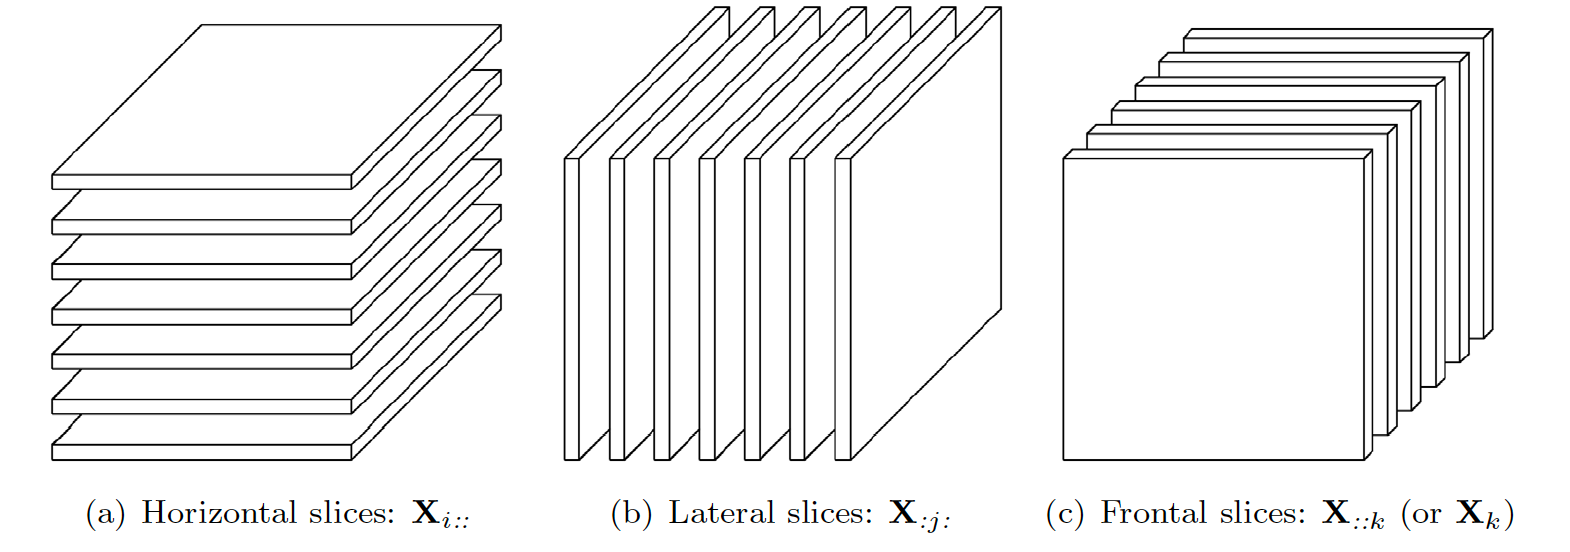
\includegraphics[keepaspectratio,width=4.8in, natwidth = 1570, natheight = 552]{figure/fig1.png}}
\caption{A visual representation of a third order tensor. It can be imagined in three distinct ways, depending on how you index it}
\label{fig_ex1.png}
\end{figure}
%%%%%%%%%%%%%%%% end figure %%%%%%%%%%%%%%%%%%%
%%%%%%%%%%%%%%%% begin figure %%%%%%%%%%%%%%%%%%%
%%% 3.34in is the maximum width you can have for a figure
\begin{figure}
\center{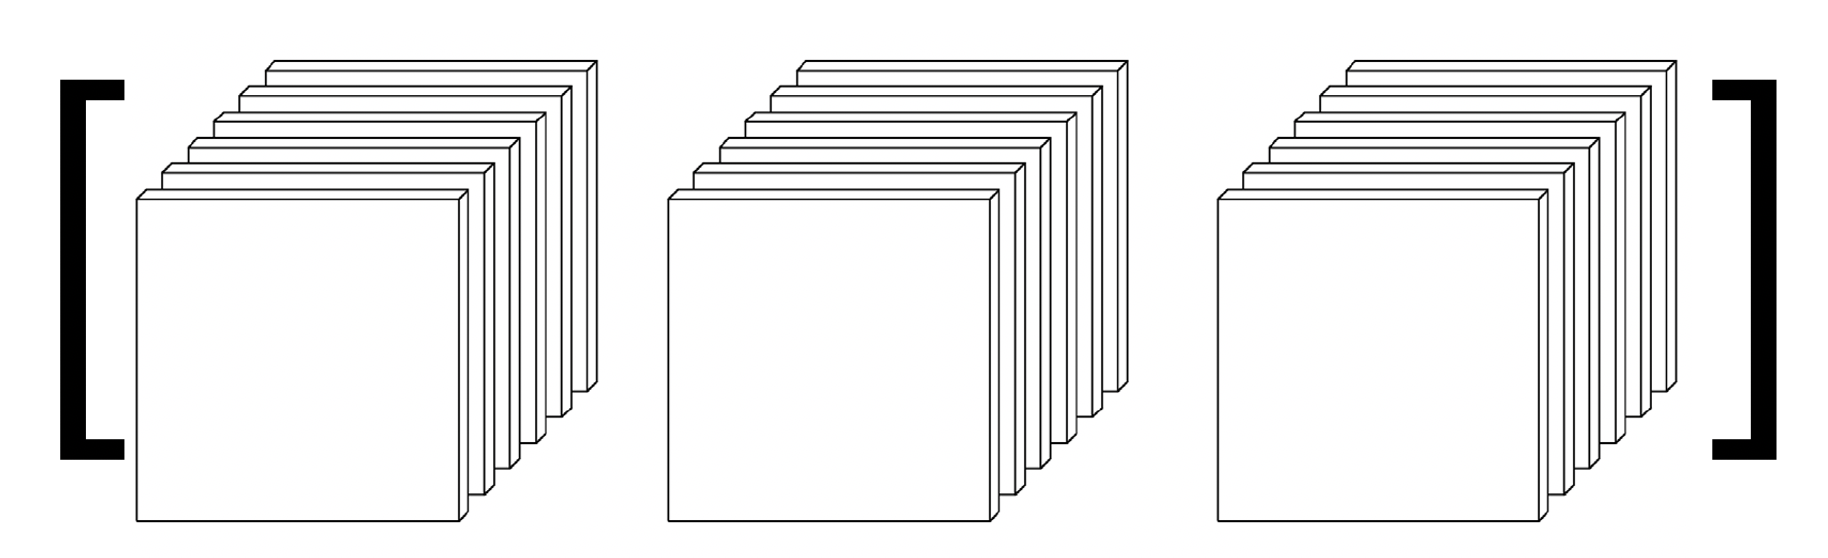
\includegraphics[keepaspectratio,width=4.8in, natwidth = 1828, natheight = 558]{figure/fig2.png}}
\caption{A visual representation of a fourth order tensor. In code, it is treated as a vector of third order tensors.}
\label{fig_ex2.png}
\end{figure}
%%%%%%%%%%%%%%%% end figure %%%%%%%%%%%%%%%%%%%

Figure~\ref{fig_ex1.png} shows a visual representation of a third order tensor; it can be imagined as a vector of matrices, where each square slice represents an individual matrix. Figure~\ref{fig_ex2.png} shows a visual representation of a fourth
order tensor, or a vector of third order tensors. Fourth order tensors are the highest dimension tensor needed for this paper, so no other tensor visuals are included.

There are three different kinds of tensor multiplication that we will use throughout this paper.

\subsection{Scalar Multiplication}

This works exactly as it seems like it would. For $a \in \mathbb{R}$, $X \in \mathbb{R}^{I_1 \times I_2 \times ... \times I_N}$,

\begin{equation}
(aX)_{i_1, i_2, ..., i_n} = a*x_{i_1, i_2, ..., i_n}
\end{equation}

%%%%%%%%%%%%%%%% begin figure %%%%%%%%%%%%%%%%%%%
%%% 3.34in is the maximum width you can have for a figure
\begin{figure}
\center{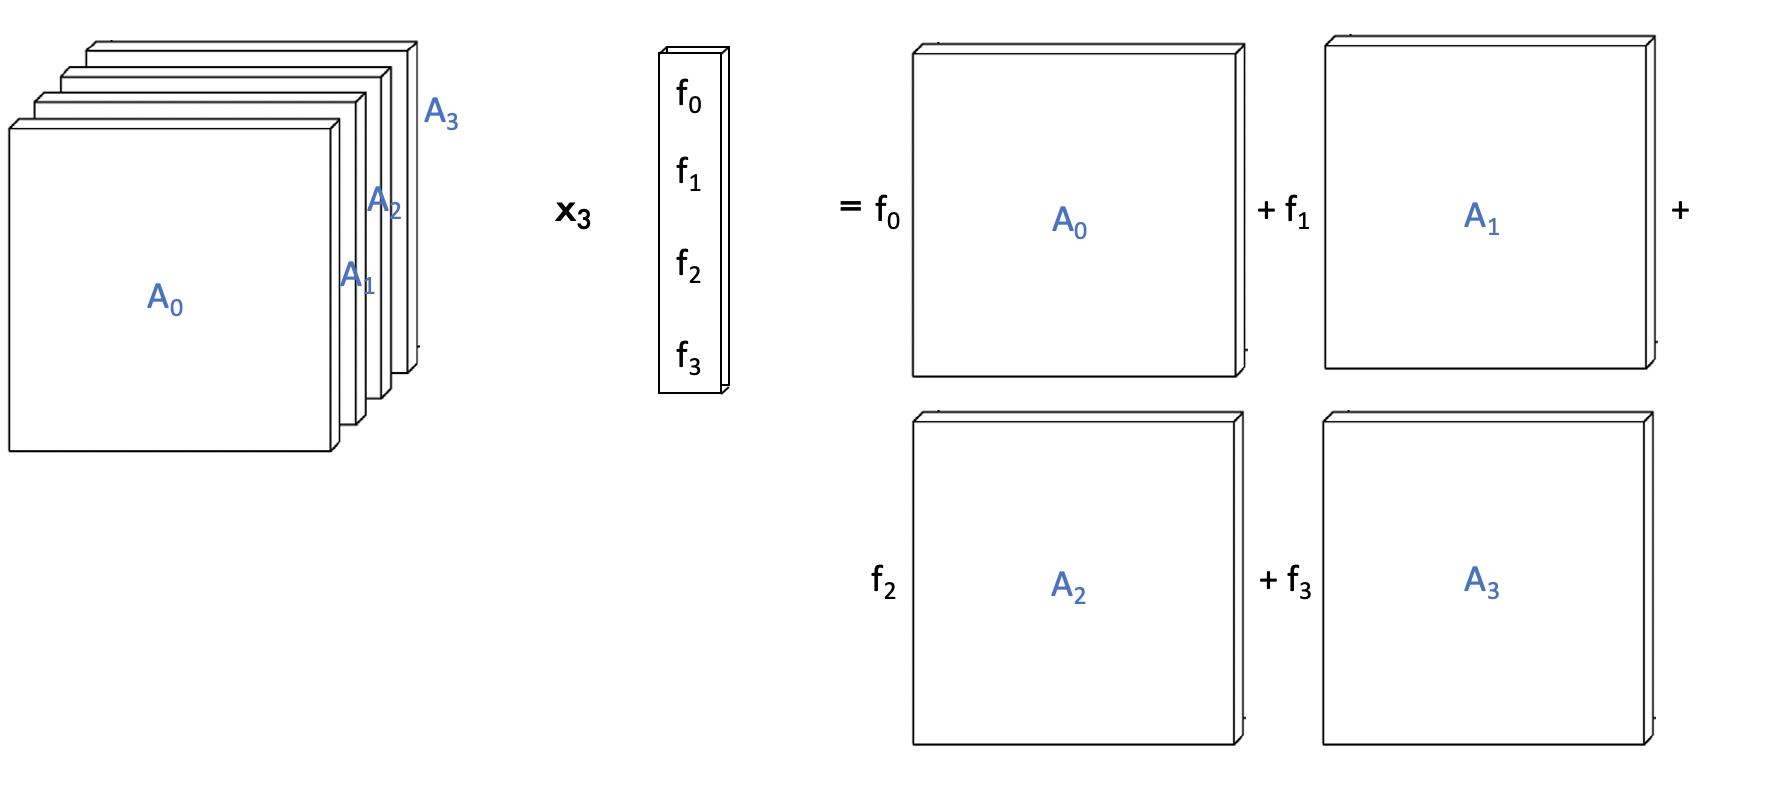
\includegraphics[keepaspectratio,width=4.8in, natwidth = 1774, natheight = 788]{figure/fig3.png}}
\caption{A visual representation of a 3-mode vector product, where $A \in \mathbb{R}^{n \times n \times 4}$ and $f \in \mathbb{R}^{4}$}
\label{fig_ex3.png}
\end{figure}
%%%%%%%%%%%%%%%% end figure %%%%%%%%%%%%%%%%%%%

\subsection{n-Mode Vector Product}

When a tensor is multiplied by a vector, its order reduces by 1. An n-mode vector product of a tensor $X \in \mathbb{R}^{I_1 \times I_2 \times ... \times I_N}$ with a vector $v \in \mathbb{R}^{I_n}$ is denoted by $X \bar{\times}_n v$. Elementwise,

\begin{equation}
(X \bar{\times}_n v )_{i_1, ..., i_{n-1}, i{n+1}, ..., i_N} = \sum_{i_n = 1}{I_n} x_{i_1, i_2, ..., i_N}*v_{i_n}
\end{equation}

So the resulting tensor $(X \bar{\times}_n v ) \in \mathbb{R}^{I_1 \times ... \times I_{n-1} \times I_{n+1} \times ... \times I_N}$. A visual representation of a 3-mode vector product can be seen in Figure~\ref{fig_ex3.png}.
For n-mode vector products, precedence matters, since it change which dimension of the tensor is collapsed. Therefore, if $m < n$,

\begin{equation}
X \bar{\times}_m a \bar{\times}_n b = (X \bar{\times}_m a) \bar{\times}_{n-1} b = (X \bar{\times}_n b) \bar{\times}_m a
\label{eq_vectorMode}
\end{equation}

This is an important rule that will be used later.

\subsection{n-Mode Matrix Product}
When a tensor is multiplied by a matrix, one of its dimensions changes. An n-mode matrix product of a tensor $X \in \mathbb{R}^{I_1 \times I_2 \times ... \times I_N}$ with a matrix $U \in \mathbb{R}^{J \times I_n}$ is denoted by $X \times_n U$. Elementwise, this multiplication results in:

\begin{equation}
(X \times_n U )_{i_1, ..., i_{n-1}, j, i{n+1}, ..., i_N} = \sum_{i_n = 1}{I_n} x_{i_1, i_2, ..., i_N}*u_{j,i_n}
\end{equation}

and the resulting tensor $(X \times_n U ) \in \mathbb{R}^{I_1 \times ... \times I_{n-1} \times J \times I_{n+1} \times ... \times I_N}$.

If $n \neq m$, then

\begin{equation}
X \times_n A \times_m  B = X \times_m B \times_n A
\label{eq_matrixModeCommute}
\end{equation}

If the modes are the same, then

\begin{equation}
X \times_n A \times_n  B = X \times_n (BA)
\label{eq_matrixModeAssociate}
\end{equation}

These two rules will also be used later.

% %%%%%%%%%%%%%%%%%%%%%%%%%%%%%%%%%%%%%%%%%%%%%%%%%%%%%%%%%%%%%%%%%%%%%%
\section{Creating the Triangles}

When modelling solids using a discrete method, the model is represented by a mesh of polygons. In this paper, triangles were
used, so all results of this paper are based on triangle calculations.

In the code for this paper, a triangle object was created for cleaner implementation. Important variables to keep track of are:
\begin{enumerate}
  \item a vector of rest vertices. This should stay constant throughout the simulation.
  \item a vector of actual positions, which update as the whole mesh moves.
  \item a material model of some sort, to keep track of lambda and mu values for force calculations.
  \item rest area; this is used in calculating the internal force and stiffness matrix.
  \item precomputed coefficients for the cubic polynomial interpretation of internal force and quadratic polynomial
  for the tangent stiffness matrix. This will be discussed in a later section.
\end{enumerate}

In addition to storing variables, there are a few useful functions that can go into this object as well:
\begin{enumerate}
  \item getter/setter functions for all private variables.
  \item a function that computes $\frac{\partial F}{\partial u}$.
  \item a function that computes the deformation gradient, $F$.
  \item a function to compute the internal force for the triangle given the deformation gradient.
  \item a function to compute the force jacobian for the triangle given the deformation gradient.
\end{enumerate}

The last three functions are not necessary for the cubic polynomial approach, but are useful for debugging purposes.
All terms used in this section will be explained in the following subsections, which will go into more details of
implementation.

% %%%%%%%%%%%%%%%%%%%%%%%%%%%%%%%%%%%%%%%%%%%%%%%%%%%%%%%%%%%%%%%%%%%%%%
\subsection{Computing the Deformation Gradient}

When a solid is deformed, the \textbf{Deformation Gradient}, $F \in \mathbb{R}^{2 \times 2}$, is the linear mapping from a rest vertex to its deformed position (without translation). This mapping can be used in the calculation of strain energy, so it's an important value to calculate if the cubic polynomial approach is not being used.

The deformation gradient can be found using the equation:

\begin{equation}
F = D_sD_{m}^{-1} = \begin{bmatrix} (x_2 - x_0) & (x_4 - x_0) \\ (x_3 - x_1) & (x_5 - x_1) \end{bmatrix} D_{m}^{-1} = \begin{bmatrix} f_0 & f_2 \\ f_1 & f_3 \end{bmatrix}
\label{eq_F}
\end{equation}

Where $D_s$ is the spatial matrix made of the deformed vertices, $D_m$ is the material matrix made of the rest vertices, and the three vertices of the triangle are $(x_0, x_1), (x_2, x_3), (x_4, x_5)$. Since the rest vertices stay constant throughout the simulation, $D_{m}^{-1}$ is constant.

% %%%%%%%%%%%%%%%%%%%%%%%%%%%%%%%%%%%%%%%%%%%%%%%%%%%%%%%%%%%%%%%%%%%%%%
\subsection{Implementing StVK}

This section is not necessary for the cubic polynomial approach, but it's useful as a debugging tool. In the code
for this paper, the implementation of StVK is tied to the material of the triangle, and is called by the functions
that calculate internal force and the force jacobian for an individual triangle.

A St. Venant-Kirchhoff deformable model is defined by the StVK strain energy, where

\begin{equation}
\psi = \mu ||F^TF - I||^2 + \frac{\lambda}{2}tr(F^TF - I)^2
\label{eq_stvk}
\end{equation}

, and $\lambda$ and $\mu$ are Lamé coefficients.

In computing the internal force of a single triangle, the Piola-Kirchhoff stress tensor, i.e. the derivative of the strain energy by the deformation gradient, is used. The Piola-Kirchhoff stress tensor is

\begin{equation}
\frac{\partial \psi}{\partial F} = 4\mu FF^TF - 4\mu F + 2\lambda Ftr(F^TF) -4\lambda F
\label{eq_pk1}
\end{equation}

In computing the force jacobian of a single triangle, the energy hessian is used. The energy hessian is:

\begin{equation}
  \begin{split}
\frac{\partial^2 \psi}{\partial F^2} = 4\mu [\frac{\partial F}{\partial F_i}F^TF + F\frac{\partial F}{\partial F_i}^TF + FF^T\frac{\partial F}{\partial F_i}] \\ + 2\lambda \frac{\partial F}{\partial F_i}tr(F^TF) - 4[\mu -\lambda]I
  \end{split}
\label{eq_dpdf}
\end{equation}

% %%%%%%%%%%%%%%%%%%%%%%%%%%%%%%%%%%%%%%%%%%%%%%%%%%%%%%%%%%%%%%%%%%%%%%
\subsection{Computing dF/dx}

Before we can calculate internal force and the force jacobian, we need to find the derivative of F in terms of x. Remember that $F \in \mathbb{R}^{2 \times 2}$ and $x \in \mathbb{R}^6$. This means that

\begin{equation}
  \begin{split}
    \frac{\partial F}{\partial x} = \begin{bmatrix} \frac{\partial F}{\partial x_0} & \frac{\partial F}{\partial x_1}
    & \frac{\partial F}{\partial x_2} & \frac{\partial F}{\partial x_3} & \frac{\partial F}{\partial x_4}
    & \frac{\partial F}{\partial x_5} \end{bmatrix} \\
    = \begin{bmatrix} \begin{bmatrix} -1 & -1 \\ 0 & 0 \end{bmatrix} & \begin{bmatrix} 0 & 0 \\ -1 & -1 \end{bmatrix}
  & \begin{bmatrix} 1 & 0 \\ 0 & 0 \end{bmatrix} & \begin{bmatrix} 0 & 0 \\ 1 & 0 \end{bmatrix}
  & \begin{bmatrix} 0 & 1 \\ 0 & 0 \end{bmatrix} & \begin{bmatrix} 0 & 0 \\ 0 & 1 \end{bmatrix}\end{bmatrix}
  \end{split}
\label{eq_dFdx}
\end{equation}

This was derived using equation~\ref{eq_F} for $F$. Notice that this is a vector of matrices, i.e. a third order tensor. While we can use this as a third order tensor, it's easier to vectorize it and treat it as a matrix.

% %%%%%%%%%%%%%%%%%%%%%%%%%%%%%%%%%%%%%%%%%%%%%%%%%%%%%%%%%%%%%%%%%%%%%%
\subsubsection{Flattening Matrices and Tensors}

Flattening a tensor reduces it into a matrix, and flattening a matrix reduces it into a vector (also called vectorizing). To vectorize a matrix, we append the next column onto the bottom of the previous. So, as an example, if

\bigskip
\begin{center}
$A = \begin{bmatrix} 1 & 3 \\ 2 & 4 \end{bmatrix}$
\end{center}

then

\begin{center}
$vec(A) = \begin{bmatrix} 1 \\ 2 \\ 3 \\ 4 \end{bmatrix}$
\end{center}

To flatten a tensor, we do this process on each level - so if we have a fourth order tensor, or a matrix of matrices, we first flatten the outer matrix into a vector of matrices, then vectorize the matrices inside. This step, which is the same for both third and fourth order tensors, can be done as shown below:

\bigskip
\begin{center}
$A = \begin{bmatrix} \begin{bmatrix} 1 & 3 \\ 2 & 4 \end{bmatrix} & \begin{bmatrix} 5 & 7 \\ 6 & 8 \end{bmatrix} \end{bmatrix}$
\end{center}

then

\begin{center}
$vec(A) = \begin{bmatrix} vec(\begin{bmatrix} 1 & 3 \\ 2 & 4 \end{bmatrix}) & vec(\begin{bmatrix} 5 & 7 \\ 6 & 8 \end{bmatrix}) \end{bmatrix} = \begin{bmatrix} 1 & 5 \\ 2 & 6 \\ 3 & 7 \\ 4 & 8 \end{bmatrix}$
\end{center}

% %%%%%%%%%%%%%%%%%%%%%%%%%%%%%%%%%%%%%%%%%%%%%%%%%%%%%%%%%%%%%%%%%%%%%%
\subsection{Computing Internal Force and the Force Jacobian (The Non-Polynomial Way)}

This section is unnecessary for the cubic polynomial approach, but as with all the other sections, it's useful for debugging purposes. The internal force inside of the triangle can be computed using the equation

\begin{equation}
f = \frac{\partial \psi}{\partial u} = vec(\frac{\partial F}{\partial x})*vec(\frac{\partial \psi}{\partial F})
\label{eq_triforce}
\end{equation}

where the terms are defined by equations \ref{eq_dFdx} and \ref{eq_pk1}, respectively. The force jacobian for each triangle can be computed using the equation

\begin{equation}
\frac{\partial^2 \psi}{\partial u^2} = vec(\frac{\partial F}{\partial x})*\frac{\partial^2 \psi}{\partial F^2}*vec(\frac{\partial F}{\partial x})^T
\label{eq_trijacob}
\end{equation}

where the terms are defined by equations \ref{eq_dFdx} and \ref{eq_dpdf}. Notice how $x$, or current vertex placement, and $u$, vertex \textit{displacement}, are used interchangably here. In general, this is possible because the interal force at rest position $\bar{x}$ is $0$, and $x = \bar{x} + u$. However, it is important to note, because these will \textbf{not} be interchangable in the cubic polynomial approach.

% %%%%%%%%%%%%%%%%%%%%%%%%%%%%%%%%%%%%%%%%%%%%%%%%%%%%%%%%%%%%%%%%%%%%%%

\section{Creating the Triangle Mesh}

Now that a triangle object has been established, a triangle mesh can be built. In the code for this paper, the triangle mesh is a separate object from the individual triangles, and it stores all of the triangles in a vector. When constructing the triangle mesh, it may be useful to store a map of each vertex to its global position, so that future calculations are easier. In this implementation, the following were stored as private variables:

\begin{enumerate}
  \item a vector of triangles, i.e. the triangle mesh.
  \item a vertex to global index mapping.
  \item a vector of vertex placements.
  \item a vector of vertex rest positions.
  \item a vector of vertex displacements.
  \item a vector of vertex indices representing which vertices are \textbf{constrained}.
  \item a vector of vertex indices representing which vertices are \textbf{unconstrained}.
  \item a vector for inteneral force.
  \item a vector for external force.
  \item a mass matrix.
  \item a vector for velocity and a vector for acceleration.
  \item the basis reduction matrix.
  \item a vector for the reduced basis vector.
\end{enumerate}

% %%%%%%%%%%%%%%%%%%%%%%%%%%%%%%%%%%%%%%%%%%%%%%%%%%%%%%%%%%%%%%%%%%%%%%
\section{Implementing the Euler-Lagrange Equation of Motion}

After setting up the triangle mesh and applying some kind of external force,the system is animated by solving the Euler-Lagrange Equation of Motion. By solving equation~\ref{eq_motion}, the displacements for the next time step can be found and added to the vertex placements. In order to do this, each term of the equation must be calculated.

% %%%%%%%%%%%%%%%%%%%%%%%%%%%%%%%%%%%%%%%%%%%%%%%%%%%%%%%%%%%%%%%%%%%%%%
\subsection{Implementing Internal Force}

While this step isn't necessary for the cubic polynomial approach, the methods are similar. In the previous section, the individual internal force for each triangle was calculated using equation~\ref{eq_triforce}. To calculate the global internal force, $R(u) \in \mathbb{R}^{2n}$, all of the individual internal forces are added up. This can be done by looping through every triangle, then looping through every vertex of the triangle. For each vertex, find where it belongs in the global context, and, if it is not constrained, add the force to the global vector. Here's an example through pseudocode below:

\begin{algorithmic}[1]
    \Function{globalInternalForce}{$null$}
        \State $global\_vector.setZero()$
        \For{triangle in triangles}
         \State $force \gets triangle.force()$
          \For{vertex in triangle vertices}
              \If {vertex is unconstrained}
                  \State $i \gets global\_index(vertex)$
                  \State add to global vector
              \EndIf
            \EndFor
        \EndFor
    \EndFunction
\end{algorithmic}

% %%%%%%%%%%%%%%%%%%%%%%%%%%%%%%%%%%%%%%%%%%%%%%%%%%%%%%%%%%%%%%%%%%%%%%
\subsection{Implementing the Tangent Stiffness Matrix}

The process here is similar to the process of calculating the global internal force. In the previous section, the individual force jacobian for each triangle was calculated using equation~\ref{eq_trijacob}. To calculate the global stiffness matrix, $K(u) \in \mathbb{R}^{2n \times 2n}$, all of the individual force jacobians are added up. This can be done by looping through every triangle, then looping through every vertex of the triangle twice. For each vertex, find where it belongs in the global context, and, if it is not constrained, add the force to the global stiffness matrix. Here's an example through pseudocode below:

\begin{algorithmic}[1]
    \Function{globalStiffnessMatrix}{$null$}
        \State $global\_stiffness.setZero()$
        \For{triangle in triangles}
         \State $jacobian \gets triangle.jacobian()$
          \For{$vertex$ in triangle vertices}
              \If {$vertex$ is unconstrained}
                  \State $i \gets global\_index(vertex)$
                  \For{$vertex_2$ in triangle vertices}
                      \If {$vertex_2$ is unconstrained}
                          \State $j \gets global\_index(vertex_2)$
                          \State add to global stiffness matrix
                      \EndIf
                    \EndFor
              \EndIf
            \EndFor
        \EndFor
    \EndFunction
\end{algorithmic}

% %%%%%%%%%%%%%%%%%%%%%%%%%%%%%%%%%%%%%%%%%%%%%%%%%%%%%%%%%%%%%%%%%%%%%%
\subsection{Implementing the Mass Matrix}

The mass matrix does not change over time, so this can be initialized outside of the motion function. How mass is implemented is up to the creator.

% %%%%%%%%%%%%%%%%%%%%%%%%%%%%%%%%%%%%%%%%%%%%%%%%%%%%%%%%%%%%%%%%%%%%%%
\subsection{Implementing the Damping Force}

The damping force is calculated using the equation

\begin{equation}
D(u, \dot u) = (\alpha M + \beta K(u)) \dot u
\label{eq_damp}
\end{equation}

After computing the global stiffness matrix, this should be straightforward. The alpha and beta values are constant values that are up to the creator, depending on how strong the desired force is.

% %%%%%%%%%%%%%%%%%%%%%%%%%%%%%%%%%%%%%%%%%%%%%%%%%%%%%%%%%%%%%%%%%%%%%%
\subsection{Implementing the Newmark Integrator}

An explanation of how to take a step in time.

% %%%%%%%%%%%%%%%%%%%%%%%%%%%%%%%%%%%%%%%%%%%%%%%%%%%%%%%%%%%%%%%%%%%%%%
\section{Generating Precomputed Coefficients}

An explanation of how to create precomputed coefficients for the cubic polynomial approach for the unreduced problem.

% %%%%%%%%%%%%%%%%%%%%%%%%%%%%%%%%%%%%%%%%%%%%%%%%%%%%%%%%%%%%%%%%%%%%%%
\subsection{Coefficients for the Tangent Stiffness Matrix}

An explanation of how to derive the coefficients for the tangent stiffness matrix equation.

% %%%%%%%%%%%%%%%%%%%%%%%%%%%%%%%%%%%%%%%%%%%%%%%%%%%%%%%%%%%%%%%%%%%%%%
\subsubsection{Constant Coefficient for the Tangent Stiffness Matrix}

An explanation of how to derive the constant coefficient for the tangent stiffness matrix.

% %%%%%%%%%%%%%%%%%%%%%%%%%%%%%%%%%%%%%%%%%%%%%%%%%%%%%%%%%%%%%%%%%%%%%%
\subsubsection{Quadratic Coefficient for the Tangent Stiffness Matrix}

An explanation of how to derive the quadratic coefficient for the tangent stiffness matrix.

% %%%%%%%%%%%%%%%%%%%%%%%%%%%%%%%%%%%%%%%%%%%%%%%%%%%%%%%%%%%%%%%%%%%%%%
\subsubsection{Creating the Global Tangent Stiffness Matrix Coefficients}

An explanation of how to derive the global tangent stiffness matrix.

% %%%%%%%%%%%%%%%%%%%%%%%%%%%%%%%%%%%%%%%%%%%%%%%%%%%%%%%%%%%%%%%%%%%%%%
\subsection{Coefficients for Internal Force}

An explanation of how to derive the coefficients for the internal force equation.

% %%%%%%%%%%%%%%%%%%%%%%%%%%%%%%%%%%%%%%%%%%%%%%%%%%%%%%%%%%%%%%%%%%%%%%
\subsubsection{Linear Coefficient for Internal Force}

An explanation of how to derive the linear coefficient for internal force.

% %%%%%%%%%%%%%%%%%%%%%%%%%%%%%%%%%%%%%%%%%%%%%%%%%%%%%%%%%%%%%%%%%%%%%%
\subsubsection{Cubic Coefficient for for Internal Force}

An explanation of how to derive the cubic coefficient for internal force.

% %%%%%%%%%%%%%%%%%%%%%%%%%%%%%%%%%%%%%%%%%%%%%%%%%%%%%%%%%%%%%%%%%%%%%%
\subsubsection{Creating the Global Internal Force Coefficients}

An explanation of how to derive the global internal force.

% %%%%%%%%%%%%%%%%%%%%%%%%%%%%%%%%%%%%%%%%%%%%%%%%%%%%%%%%%%%%%%%%%%%%%%
\section{Generating a Deformation Basis}

An explanation of how to generate a deformation basis.

% %%%%%%%%%%%%%%%%%%%%%%%%%%%%%%%%%%%%%%%%%%%%%%%%%%%%%%%%%%%%%%%%%%%%%%
\section{Reducing the Euler-Lagrange Equation of Motion}

An explanation of how to push U through so that we can reduce the order of our calculations.

% %%%%%%%%%%%%%%%%%%%%%%%%%%%%%%%%%%%%%%%%%%%%%%%%%%%%%%%%%%%%%%%%%%%%%%
\subsection{Reducing the Internal Force}

An explanation of how to reduce the calculation of the internal forces, changing the coefficients
of the polynomial.

% %%%%%%%%%%%%%%%%%%%%%%%%%%%%%%%%%%%%%%%%%%%%%%%%%%%%%%%%%%%%%%%%%%%%%%
\subsection{Reducing the Global Tangent Stiffness Matrix}

An explanation of how to reduce the calculation of the stiffness, changing the coefficients
of the polynomial.

% %%%%%%%%%%%%%%%%%%%%%%%%%%%%%%%%%%%%%%%%%%%%%%%%%%%%%%%%%%%%%%%%%%%%%%
\subsection{Reducing All Other Forces}

An explanation of how to reduce all other forces.

% %%%%%%%%%%%%%%%%%%%%%%%%%%%%%%%%%%%%%%%%%%%%%%%%%%%%%%%%%%%%%%%%%%%%%%
\section{Running the program}

A brief explanation of how to run the program

% %%%%%%%%%%%%%%%%%%%%%%%%%%%%%%%%%%%%%%%%%%%%%%%%%%%%%%%%%%%%%%%%%%%%%%
\section{Conclusions}

End it by explaining how I hope this helps anyone who wants to try implementing this on their own.
Explain how this can probably be optimized further by flattening all tensors.

% %%%%%%%%%%%%%%%%%%%%%%%%%%%%%%%%%%%%%%%%%%%%%%%%%%%%%%%%%%%%%%%%%%%%%%
\begin{acknowledgment}

Thanks to Barbič for writing the paper and my advisor Theodore Kim.

\end{acknowledgment}

%%%%%%%%%%%%%%%%%%%%%%%%%%%%%%%%%%%%%%%%%%%%%%%%%%%%%%%%%%%%%%%%%%%%%%

% % %%%%%%%%%%%%%%%%%%%%%%%%%%%%%%%%%%%%%%%%%%%%%%%%%%%%%%%%%%%%%%%%%%%%%%
% \section{Footnotes\protect\footnotemark}
% \footnotetext{Examine the input file, asme2ej.tex, to see how a footnote is given in a head.}
%
% Footnotes are referenced with superscript numerals and are numbered consecutively from 1 to the end of the paper\footnote{Avoid footnotes if at all possible.}. Footnotes should appear at the bottom of the column in which they are referenced.


% %%%%%%%%%%%%%%%%%%%%%%%%%%%%%%%%%%%%%%%%%%%%%%%%%%%%%%%%%%%%%%%%%%%%%%
% \section{Mathematics}
%
% Equations should be numbered consecutively beginning with (1) to the end of the paper, including any appendices.  The number should be enclosed in parentheses and set flush right in the column on the same line as the equation.  An extra line of space should be left above and below a displayed equation or formula. \LaTeX\ can automatically keep track of equation numbers in the paper and format almost any equation imaginable. An example is shown in Eqn.~(\ref{eq_ASME}). The number of a referenced equation in the text should be preceded by Eqn.\ unless the reference starts a sentence in which case Eqn.\ should be expanded to Equation.
%
% \begin{equation}
% f(t) = \int_{0_+}^t F(t) dt + \frac{d g(t)}{d t}
% \label{eq_ASME}
% \end{equation}
%
% %%%%%%%%%%%%%%%%%%%%%%%%%%%%%%%%%%%%%%%%%%%%%%%%%%%%%%%%%%%%%%%%%%%%%%
% \section{Figures}
% \label{sect_figure}
%
% All figures should be positioned at the top of the page where possible.  All figures should be numbered consecutively and centered under the figure as shown in Fig.~\ref{figure_ASME}. All text within the figure should be no smaller than 7~pt. There should be a minimum two line spaces between figures and text. The number of a referenced figure or table in the text should be preceded by Fig.\ or Tab.\ respectively unless the reference starts a sentence in which case Fig.\ or Tab.\ should be expanded to Figure or Table.
%
%
% %%%%%%%%%%%%%%%%%%%%%%%%%%%%%%%%%%%%%%%%%%%%%%%%%%%%%%%%%%%%%%%%%%%%%%
% %%%%%%%%%%%%%%%% begin figure %%%%%%%%%%%%%%%%%%%
% \begin{figure}[t]
% \begin{center}
% \setlength{\unitlength}{0.012500in}%
% \begin{picture}(115,35)(255,545)
% \thicklines
% \put(255,545){\framebox(115,35){}}
% \put(275,560){Beautiful Figure}
% \end{picture}
% \end{center}
% \caption{The caption of a single sentence does not have period at the end}
% \label{figure_ASME}
% \end{figure}
% %%%%%%%%%%%%%%%% end figure %%%%%%%%%%%%%%%%%%%
% %%%%%%%%%%%%%%%%%%%%%%%%%%%%%%%%%%%%%%%%%%%%%%%%%%%%%%%%%%%%%%%%%%%%%%
%
% In the following subsections, I have inserted figures that have been provided by authors in order to demonstrate what to avoid.  In each case the authors provided figures that are 3.25in wide and 600dpi in the .tif graphics format.  The papers containing these figures have been held from production due to their poor quality.
%
% %%%%%%%%%%%%%%%%%%%%%%%%%%%%%%%%%%%%%%%%%%%%%%%%%%%%%%%%%%%%%%%%%%%%%%
% \subsection{The 1st Example of Bad Figure}
%
% %%%%%%%%%%%%%%%% begin figure %%%%%%%%%%%%%%%%%%%
% %%% 3.34in is the maximum width you can have for a figure
% \begin{figure}
% \centerline{\psfig{figure=figure/FMANU_MD_05_1107_11.ps,width=3.34in}}
% \caption{Example taken from a paper that was held from production because the image quality is poor.  ASME sets figures captions in 8pt, Helvetica Bold.}
% \label{fig_example1.ps}
% \end{figure}
% %%%%%%%%%%%%%%%% end figure %%%%%%%%%%%%%%%%%%%
%
% In order to place the figure in this template using MSWord, select ����Insert Picture from File,���� and use wrapping that is  ����top and bottom.����  Make sure the figure is 3.25in wide.
%
% Figure~`\ref{fig_example1.ps}
% was taken from a recent paper that was held from publication, because the text is fuzzy and unreadable.  It was probably obtained by taking a screen shot of the computer output of the author����s software.  This means the original figure was 72dpi (dots per inch) on a computer screen.  There is no way to improve the quality such a low resolution figure.
%
% In order to understand how poor the quality of this figure is, please zoom in slightly, say to 200\%.  Notice that while the font of the paper is clear at this size, the font in the figures is fuzzy and blurred.  It is impossible to make out the small symbol beside the numbers along the abscissa of the graph.  Now consider the labels ����Time���� and ����Cost.����  They are clearly in fonts larger that the text of the article, yet the pixilation or rasterization, associated with low resolution is obvious. This figure must be regenerated at higher resolution to ensure quality presentation.
%
% The poor quality of this figure is immediately obvious on the printed page, and reduces the impact of the research contribution of the paper, and in fact detracts from the perceived quality of the journal itself.
%
%
%
% %%%%%%%%%%%%%%%%%%%%%%%%%%%%%%%%%%%%%%%%%%%%%%%%%%%%%%%%%%%%%%%%%%%%%%
% \subsection{The 2nd Example of Bad Figure}
%
% %%%%%%%%%%%%%%%% begin figure %%%%%%%%%%%%%%%%%%%
% \begin{figure}
% \centerline{\psfig{figure=figure/FMANU_MD_05_1272_5.ps,width=3.34in}}
% \caption{While this figures is easily readable at a double column width of 6.5in, when it is shrunk to 3.25in column width the text is unreadable.   This paper was held from production.}
% \label{fig_example2.ps}
% \end{figure}
% %%%%%%%%%%%%%%%% end figure %%%%%%%%%%%%%%%%%%%
%
% Figure~\ref{fig_example2.ps}
% demonstrates a common problem that arises when a figure is scaled down fit a single column width of 3.25in.  The original figure had labels that were readable at full size, but become unreadable when scaled to half size.  This figure also suffers from poor resolution as is seen in the jagged lines the ovals that form the chain.
%
% This problem can be addressed by increasing the size of the figure to a double column width of 6.5in, so the text is readable.  But this will not improve the line pixilation, and a large low resolution figure is less desirable than a small one.  This also significantly expands the length of the paper, and may cause it to exceed the JMD nine page limit.  Additional pages require page charges of \$200 per page.  It is best to regenerate the figure at the resolution that ensures a quality presentation.
%
%
% %%%%%%%%%%%%%%%%%%%%%%%%%%%%%%%%%%%%%%%%%%%%%%%%%%%%%%%%%%%%%%%%%%%%%%
% \subsection{The 3rd Example of Bad Figure}
% %%%%%%%%%%%%%%%% begin figure %%%%%%%%%%%%%%%%%%%
% \begin{figure}
% %\centerline{\psfig{figure=figure/FMANU_MD_04_1274_13.ps,width=3.34in}}
% \centerline{\psfig{figure=figure/FMANU_MD_04_1274_13.ps,width=3.25in}}
% \caption{Another example of a figure with unreadable text.  Even when the paper was expanded to double column width the text as shown in Fig.~\ref{fig_example4.ps} was of such low quality that the paper was held from production.}
% \label{fig_example3.ps}
% \end{figure}
% %%%%%%%%%%%%%%%% end figure %%%%%%%%%%%%%%%%%%%
%
% %%%%%%%%%%%%%%%% begin figure %%%%%%%%%%%%%%%%%%%
% %%% the maximum width in double column is 6.85in
% \begin{figure*}
% \centerline{\psfig{figure=figure/FMANU_MD_04_1274_13.ps,width=6.85in}}
% \caption{A figure expanded to double column width the text from Figure~\ref{fig_example3.ps}}
% \label{fig_example4.ps}
% \end{figure*}
% %%%%%%%%%%%%%%%% end figure %%%%%%%%%%%%%%%%%%%
% An author provided the high resolution image
% in Fig.~\ref{fig_example3.ps}
% that was sized to a single column width of 3.25in.  Upon seeing the poor quality of the text, the publisher scaled the image to double column width as shown in Fig.~\ref{fig_example4.ps}
% at which point it took half of a page.  The publisher went on to do this for all eight figures generating four pages of figures that the author did not expect. ASME stopped production of the paper even with the larger figures due to the pixilation of the font.
%
% Clearly the text in this figure is unreadable, and it is doubtful that the author can print the output in a way that it is readable.  This is a problem that the author must solve, not the publisher.
%
% As you might expect, I have many more examples, but in the end the author is the best judge of what is needed in each figure.  ASME simply requires that the image meet a minimum standard for font and line quality, specifically the font should be the appropriate size and not be blurred or pixilated, and that lines should be the appropriate weight and have minimal, preferably no, pixilation or rasterization.
%
%
% %%%%%%%%%%%%%%%%%%%%%%%%%%%%%%%%%%%%%%%%%%%%%%%%%%%%%%%%%%%%%%%%%%%%%%
% \section{Tables}
%
% %%%%%%%%%%%%%%%%%%%%%%%%%%%%%%%%%%%%%%%%%%%%%%%%%%%%%%%%%%%%%%%%%%%%%%
% %%%%%%%%%%%%%%% begin table   %%%%%%%%%%%%%%%%%%%%%%%%%%
% \begin{table}[t]
% \caption{Figure and table captions do not end with a period}
% \begin{center}
% \label{table_ASME}
% \begin{tabular}{c l l}
% & & \\ % put some space after the caption
% \hline
% Example & Time & Cost \\
% \hline
% 1 & 12.5 & \$1,000 \\
% 2 & 24 & \$2,000 \\
% \hline
% \end{tabular}
% \end{center}
% \end{table}
% %%%%%%%%%%%%%%%% end table %%%%%%%%%%%%%%%%%%%
% %%%%%%%%%%%%%%%%%%%%%%%%%%%%%%%%%%%%%%%%%%%%%%%%%%%%%%%%%%%%%%%%%%%%%%
%
% All tables should be numbered consecutively  and centered above the table as shown in Table~\ref{table_ASME}. The body of the table should be no smaller than 7 pt.  There should be a minimum two line spaces between tables and text.
%
%
% %%%%%%%%%%%%%%%%%%%%%%%%%%%%%%%%%%%%%%%%%%%%%%%%%%%%%%%%%%%%%%%%%%%%%%
% \section{Citing References}
%
% %%%%%%%%%%%%%%%%%%%%%%%%%%%%%%%%%%%%%%%%%%%%%%%%%%%%%%%%%%%%%%%%%%%%%%
% The ASME reference format is defined in the authors kit provided by the ASME.  The format is:
%
% \begin{quotation}
% {\em Text Citation}. Within the text, references should be cited in  numerical order according to their order of appearance.  The numbered reference citation should be enclosed in brackets.
% \end{quotation}
%
%
% The bibliography style required by the ASME is unsorted with entries appearing in the order in which the citations appear. If that were the only specification, the standard {\sc Bib}\TeX\ unsrt bibliography style could be used. Unfortunately, the bibliography style required by the ASME has additional requirements (last name followed by first name, periodical volume in boldface, periodical number inside parentheses, etc.) that are not part of the unsrt style. Therefore, to get ASME bibliography formatting, you must use the \verb+asmems4.bst+ bibliography style file with {\sc Bib}\TeX. This file is not part of the standard BibTeX distribution so you'll need to place the file someplace where LaTeX can find it (one possibility is in the same location as the file being typeset).
%
% With \LaTeX/{\sc Bib}\TeX, \LaTeX\ uses the citation format set by the class file and writes the citation information into the .aux file associated with the \LaTeX\ source. {\sc Bib}\TeX\ reads the .aux file and matches the citations to the entries in the bibliographic data base file specified in the \LaTeX\ source file by the \verb+\bibliography+ command. {\sc Bib}\TeX\ then writes the bibliography in accordance with the rules in the bibliography .bst style file to a .bbl file which \LaTeX\ merges with the source text.  A good description of the use of {\sc Bib}\TeX\ can be found in \cite{latex, goosens} (see how two references are handled?).  The following is an example of how three or more references \cite{latex, asmemanual,  goosens} show up using the \verb+asmems4.bst+ bibliography style file in conjunction with the \verb+asme2ej.cls+ class file. Here are some more \cite{art, blt, ibk, icn, ips, mts, mis, pro, pts, trt, upd} which can be used to describe almost any sort of reference.
%

% Here's where you specify the bibliography style file.
% The full file name for the bibliography style file
% used for an ASME paper is asmems4.bst.
\bibliographystyle{asmems4}

% Here's where you specify the bibliography database file.
% The full file name of the bibliography database for this
% article is asme2e.bib. The name for your database is up
% to you.
\bibliography{writeup}

\end{document}
